\documentclass{book}
\usepackage{listings}
\usepackage{hyperref}
\usepackage{verbatim}
\usepackage{amsmath}
\usepackage[backend=bibtex, sorting=none, style=numeric-comp, defernumbers]{biblatex}
\usepackage{graphicx}

\addbibresource{\jobname.bib}

\begin{document}

\title{Chapter 2 - Rust Machine Learning}
\author {Joydeep Bhattacharjee}

\maketitle

\section{What is machine learning}
Machine learning is the science of getting computers to act without being specifically programmed. This is done by implementing special algorithms that have the ability to detect patterns in data. From a developer point of view this means creating a system, which has access to relevant data, is able to feed the data to machine learning algorithms and is able to take the output and redirect it to downstream processes and tasks.

\section{Supervised learning}%

Supervised learning happens when you pass both the input and the desired outputs to the system and you want the resulting machine learning model to capture the relationship. Supervised learning are again divided into two subsections based on the type of the labels.

Supervised tasks when the target variable is continuous are termed as regression problems. For example the price of a product can be any value. We should probably go for regression techniques when the prediction needs to be made on something that requires the prediction of a quantity of some sort. Quality of a regression model is generally measured using some form of error measures, that is the difference between the target values and the predicted values.

Classifications problems are different from regression problems in that the labels are discrete and finite. For example, we can categorize an email message as spam or ham. So a problem is a classification problem when we are interested in the resulting bucket that a particular set of feature readings will fall into. Quality of a classification model is generally measured using an accuracy measure which is essentially the count of the number of times the model has been right.

In this chapter we will be taking a look at implementing different regression algorithms using Rust. We will first read a data set from a csv file. This is a common data set and will be representative of the types of data in the real world. Then we will look at the logic of different popular regression algorithms, why they work and how to implement them using some Rust ML packages such as \lstinline{rusty_machine}. We will end the chapter with methods of evaluating regression models.

By the end of this chapter you should have a fair understanding of how to create common regression models and implement them in Rust.

\label{sec:supervised_learning}

\section{Dataset specific code}%
Before going into regression algorithms and the associated code lets build the surrounding boilerplate code. Look at the $rusty\_machine\_regression$ package for the accompanying code in this.

For showing usage of regression we will be using the boston housing dataset\footnote{\href{https://www.cs.toronto.edu/~delve/data/boston/bostonDetail.html}{Housing dataset source}}. The dataset has 14 features and has 506 cases. Below is a description of the dataset.

\begin{itemize}
	\item CRIM - per capita crime rate by town
	\item ZN - proportion of residential land zoned for lots over 25,000 sq.ft.
	\item INDUS - proportion of non-retail business acres per town.
	\item CHAS - Charles River dummy variable (1 if tract bounds river; 0 otherwise)
	\item NOX - nitric oxides concentration (parts per 10 million)
	\item RM - average number of rooms per dwelling
	\item AGE - proportion of owner-occupied units built prior to 1940
	\item DIS - weighted distances to five Boston employment centres
	\item RAD - index of accessibility to radial highways
	\item TAX - full-value property-tax rate per \$10,000
	\item PTRATIO - pupil-teacher ratio by town
	\item B - 1000(Bk - 0.63)\^2 where Bk is the proportion of blacks by town
	\item LSTAT - \% lower status of the population
	\item MEDV - Median value of owner-occupied homes in \$1000's.
\end{itemize}

The data is kept in a file "data/housing.csv". A quick look at the csv suggests that it is a fixed width files with no headers.

\begin{lstlisting}[language=bash,caption={housing data}]
$ head -n1 data/housing.csv \
   | grep -Eo '[0-9]*[.]?[0-9]*' \
   | wc -l
14
$ head -n2 data/housing.csv
 0.00632  18.00   2.310  0  0.5380  6.5750  65.20  4.0900   1  296.0  15.30 396.90   4.98  24.00
 0.02731   0.00   7.070  0  0.4690  6.4210  78.90  4.9671   2  242.0  17.80 396.90   9.14  21.60
\end{lstlisting}

To parse through the files we will need these dependencies in our \lstinline{Cargo.toml} file.

\begin{lstlisting}[caption={Cargo.toml}]
[dependencies]
serde = "1"
serde_derive = "1"
rand = "0.6.5"
\end{lstlisting}

\paragraph{}%
And we will need to import the required modules in the module. Most of the code in this book has been written in Rust 2018 and hence we will not need explicit \lstinline{extern} crate statements for all the dependencies.
\label{par:import_required_modules}

\begin{lstlisting}[caption={regression}]
extern crate serde;
#[macro_use]
extern crate serde_derive;
use std::io::prelude::*;
use std::io::BufReader;
use std::path::Path;
use std::fs::File;
use std::vec::Vec;
use std::error::Error;
use rand::thread_rng;
use rand::seq::SliceRandom;

\end{lstlisting}

\paragraph{}%
To parse the file and match with appropriate records we create a \lstinline{struct} with each value to be a \lstinline{float64}\footnote{This does not mean that they cannot be used in 32-bit machines. Floats have nothing to do with the bitness of the machine.}. We will need to initialise them as \lstinline{float64} due to the Rust machine learning library to we will use that we will introduce later in this section.
\label{par:}

\begin{lstlisting}[caption={chapter2\\/ml\\-utils\\/src\\/datasets\\.rs}]
struct BostonHousing {
  crim: f64, cazn: f64, indus: f64, chas: f64, nox: f64,
  rm: f64, age: f64, dis: f64, rad: f64, tax: f64,
  ptratio: f64, black: f64, lstat: f64, medv: f64,
}
\end{lstlisting}

\paragraph{}%
One way to convert the file into records is to read the file line by line and build the \lstinline{BostonHousing} record. This should enable us to implement methods that separate out the features and the labels. In this case we consider the median value of the house or the price of the house as the label and we will try to predict the price of the house based on the other features available.
\label{par:}

\paragraph{}%
Below is the code to implement the building of a \lstinline{BostonHousing} record and methods to build the feature vector and label.
\label{par:}

\begin{lstlisting}[caption={chapter2\\/ml\\-utils\\/src\\/datasets\\.rs}]
impl BostonHousing {
  fn new(v: Vec<&str>) -> BostonHousing {
    let n: Vec<f64> = v.iter().map(
      |s| s.parse().unwrap()).collect();
  BostonHousing { crim: n[0], zn: n[1],
    indus: n[2], chas: n[3], nox: n[4],
    rm: n[5], age: n[6], dis: n[7],
    rad: n[8], tax: n[9], ptratio: n[10],
    black: n[11], lstat: n[12], medv: n[13] }
  }

  fn into_feature_vector(&self) -> Vec<f64> {
    vec![self.crim, self.zn, self.indus, self.chas, self.nox,
      self.rm, self.age, self.dis, self.rad,
      self.tax, self.ptratio, self.black, self.lstat]
  }

  fn into_labels(&self) -> f64 {
    self.medv
  }
}
\end{lstlisting}

\paragraph{}%
Now that we can proceed and start reading the file line by line using \lstinline{get_boston_records_from_file }. Each line will be passed to the \lstinline{get_boston_record} function which splits the string to a vector of strings to be parsed appropriately by \lstinline{BostonRecord}. We assign this to a mutable variable data to be used later.
\label{par:}

\begin{lstlisting}[caption={chapter2\\/ml\\-utils\\/src\\/datasets\\.rs}]
fn get_boston_record(s: String) -> BostonHousing {
  let v: Vec<&str> = s.split_whitespace().collect();
  let b: BostonHousing = BostonHousing::new(v);
  b
}

fn get_boston_records_from_file(
    fl: impl AsRef<Path>) -> Vec<BostonHousing> {
  let file = File::open(fl).expect("no such file");
  let buf = BufReader::new(file);
  buf.lines().enumerate()
    .map(|(n, l)| l.expect(
       &format!("Could not parse line no {}", n)))
    .map(|r| get_boston_record(r))
    .collect()
}
\end{lstlisting}


We should now be able to call the function in our code.

\begin{lstlisting}[caption={chapter2\\/rustlymachine\_regression\\/src\\/lin\_reg\\.rs}]
use ml_utils::datasets::get_boston_records_from_file;

let fl = "data/housing.csv";
let mut data = get_boston_records_from_file(&fl);
\end{lstlisting}

\paragraph{}%
In machine learning tasks it is a good practice to shuffle the incoming dataset. Shuffling data serves the purpose of reducing variance and making sure that models remain general and overfit less. Shuffling helps in making sure that the train/test/validation samples of the dataset are representative of the overall distribution of the data.
\label{par:}

\paragraph{}%
Below we shuffle the data, split them into 80\% train and 20\% test and convert them into \lstinline{f64} vectors.
\label{par:}

\begin{lstlisting}[caption={chapter2\\/rustlymachine\_regression\\/src\\/lin\_reg\\.rs}]
data.shuffle(&mut thread_rng());

// separate out to train and test datasets.
let test_size: f64 = 0.2;
let test_size: f64 = data.len() as f64 * test_size;
let test_size = test_size.round() as usize;
let (test_data, train_data) = data.split_at(test_size);
let train_size = train_data.len();
let test_size = test_data.len();

// differentiate the features and the labels.
let boston_x_train: Vec<f64> = train_data.iter()
  .flat_map(|r| r.into_feature_vector())
  .collect();
let boston_y_train: Vec<f64> = train_data.iter()
  .map(|r| r.into_labels()).collect();
let boston_x_test: Vec<f64> = test_data.iter()
  .flat_map(|r| r.into_feature_vector()).collect();
let boston_y_test: Vec<f64> = test_data.iter()
  .map(|r| r.into_labels()).collect();
\end{lstlisting}

All of the above code has been kept in the \lstinline{datasets} module of the \lstinline{ml-utils} package.

\label{sub:dataset_specific_code}

\section{Rusty Machine Library}%

\paragraph{}%
Rusty machine is a general purpose machine learning library written entirely in Rust. The main aims of rusty-machine are ease of use and speed without having to depend on a huge number of external libraries. The consistency in the api is achieved using Rust’s trait system. It currently uses \lstinline{rulinalg} for its linear algebra backend. In this book one of the core libraries that we will focus on to achieve our machine learning needs is by using this library.
\label{par:}

\paragraph{}%
To use the rusty-machine library we will need to convert the data vectors into \lstinline{rulianalg} supported Matrices. Convert the above vectors like below.
\label{par:}

\begin{lstlisting}[caption={chapter2\\/rustlymachine\_regression\\/src\\/lin\_reg\\.rs}]
use rusty_machine;
use rusty_machine::linalg::Matrix;
use rusty_machine::linalg::Vector;

let boston_x_train = Matrix::new(train_size, 13, boston_x_train);
let boston_y_train = Vector::new(boston_y_train);
let boston_x_test = Matrix::new(test_size, 13, boston_x_test);
let boston_y_test = Matrix::new(test_size, 1, boston_y_test);
\end{lstlisting}

\paragraph{}%
In rusty-machine the two key methods that are implemented throughout is the \lstinline{train} and \lstinline{predict} methods.
\label{par:}

\label{sub:rusty_machine_library}

\section{Linear Regression with OLS and Gradient Descent}%

\paragraph{}%
Ordinary Least Squares linear regression is the method where a linear model with coefficients $w = (w1, w2, \dots, wp)$ to minimise the residual sum of squares between the observed responses in the dataset, and the responses predicted by the linear approximation. Mathematically it solves the problem of the form:
\label{par:}

\begin{equation}
	\underset{\omega}{\min} = || X\omega - y ||^2
\end{equation}

\paragraph{}%
To optimise the model one of the methods is Gradient Descent. It is a first order iterative approach to finding the minimum of a function. The update to the parameters are proportional to the negative of the gradient of the function at the current point. Rusty-machine implements batch gradient descent currently for OLS which can be implemented using the following code. In batch learning the cost is calculated for the entire dataset and for each iteration of the gradient descent algorithm.
\label{par:}

\paragraph{}%
Train a linear regression model using the below code.
\label{par:}

\begin{lstlisting}[caption={chapter2\\/rustlymachine\_regression\\/src\\/lin\_reg\\.rs}]
let mut lin_model = LinRegressor::default();
lin_model.train(&boston_x_train, &boston_y_train)?;
\end{lstlisting}

Creating a linear regression model similar to above is kept in the module \lstinline{chapter2/rustlymachine_regression/src/lin_reg.rs} module.

\label{sub:linear_regression_with_ols_and_gradient_descent}

\section{Gaussian Process}%
\paragraph{}%
Gaussian Processes can be used in regression problems. One can think of a Gaussian process as defining distribution over functions, and inference taking place directly in the space of functions, the function-space view. The predictions from a Gaussian Process model take the form of a full predictive distribution. Thus a Gaussian  process is a collection of random variables, any finite number of which have a joint Gaussian distribution.
\label{par:}
\paragraph{}%
A Gaussian Process is completely specified by its mean function and covariance function. Lets take a mean function and covariance function as below,
\label{par:paragraph_name}
\begin{align}
	m(x) & = E[f(x)],	\\
	k(x, x') & = E[(f(x) - m(x))(f(x') - m(x'))]
\end{align}

And we will write the Gaussian Process as

\begin{equation}
	f(x) \sim GP(m(x), k(x, x'))
\end{equation}

\paragraph{}%
Thus the priors of a GP needs to be specified. Generally the prior is assumed to be zero or the mean of the dataset. The priors covariance is specified by passing a kernel object.
\label{par:}

\paragraph{}%
The noise levels of the Gaussian process can also be passed. A moderate noise level can be helpful for dealing with numeric issues when fitting as it is effectively implemented as Tikhonov regularisation, ie. by adding it to the diagonal of the kernel matrix.
\label{par:}

The advantages of the Gaussian process are:

\begin{itemize}
	\item The predictions interpolates the observations for regular kernels.
	\item The prediction is probabilistic and so computing empirical confidence intervals is possible and we are able to decide based on those if one should retrofit the prediction in some region of interest for example in online or adaptive fitting.
	\item Different kernels can be specified. We can create our own kernels and apply GP using them.
\end{itemize}

The disadvantages are:

\begin{itemize}
	\item They are not sparse and they need all the information in memory to make the predictions.
	\item They lose efficiency in high dimensional spaces.
\end{itemize}

\paragraph{}%
Create a Gaussian process model to train it on the train dataset above. Here a kernel with lengthscale 2 and amplitude 1 is defined as the covariance function. A Zero function is defined as the mean function and noise levels is clipped at 10.0. We then pass the training x’s and y’s to the train method. This optimises the model according to the training values.
\label{par:}


\begin{lstlisting}[caption={gaussian\_process\_reg\\.rs}]
use rusty_machine::learning::gp::GaussianProcess;
use rusty_machine::learning::gp::ConstMean;
use rusty_machine::learning::toolkit::kernel;
use rusty_machine::learning::SupModel;

let ker = kernel::SquaredExp::new(2., 1.);
let zero_mean = ConstMean::default();
let mut gaus_model = GaussianProcess::new(ker, zero_mean, 10f64);
gaus_model.train(&boston_x_train, &boston_y_train)?;
\end{lstlisting}

Creating a Gaussian process model similar to above is kept in the module \lstinline{chapter2/rustlymachine_regression/src/gaussian_process_reg.rs} module.

\label{sub:gaussian_process}

\section{Generalized Linear Models}%
\paragraph{}%
Ordinary linear regression assumed that the unknown quantity is the linear combination of the set of predictors. This assumption is fine if the response variable is a normal distribution of the input variables. Such data can be any kind of data that is relatively stable and varies by a small amount. This can be seen in many natural distributions such as the heights of human beings where one value is independent of another value and hence central limit theorem is able to play a role. In real life though many distributions are not normal.


The generalised linear model is a flexible variation of the OLS Regression model that allows for response variables that have error distribution models other than normal distribution. In these models, the response variable $y_i$ is assumed to follow an exponential family distribution of mean $\mu_i$, which is assumed to be some (linear or non linear) function of $x_i^T\beta$\cite{WEBSITE:2}.

The GLM consists of three elements\cite{WEBSITE:3} 

\begin{enumerate}
	\item A linear predictor similar to OLS.
		\begin{equation}
			\eta_i = \beta_0 + \beta_1 x_{1i} + \dots + \beta_p x_{pi}
		\end{equation}
		or in matrix form $\eta = X \beta$

	\item A link function that describes how the mean, $E(Y_i) = \mu_i$ depends on the linear predictor
		\begin{equation}
			g(\mu_i) = \eta_i
		\end{equation}
	\item A variance function that describes how the variance, var($Y_i$) depends on the mean,
		\begin{equation}
			\text{var}(Y_i) = \phi V(\mu)
		\end{equation}
\end{enumerate}

It is convenient if V follows an exponential family of distributions. The unknown parameters $\beta$ are typically estimated using maximum likelihood, maximum-quasi likelihood or Bayesian methods. It can be shown that the general linear model is a special case of the GLM where the link function is $g(\mu_i) = \mu_i$ and the variance function is $V(\mu_i) = 1$.

In rusty machine we can create a linear regression model using the below code.

\begin{lstlisting}{caption=glms.rs}
// Create a normal generalised linear model
let mut normal_model = GenLinearModel::new(Normal);
normal_model.train(&boston_x_train, &boston_y_train)?;

let predictions = normal_model.predict(&boston_x_test).unwrap();
let predictions = Matrix::new(test_size, 1, predictions);
let acc = neg_mean_squared_error(&predictions, &boston_y_test);
\end{lstlisting}

Other models that are implemented are Bernoulli and Binomial which are mainly used for classification. We can also use Poisson regression for the Criterion. Poisson regression is similar to multiple regression except that the dependent variable is an observed count that follows the Poisson distribution. Thus the possible values of Y are non-negative integers: $0, 1, \dots$ and so on. It is assumed that the large counts are rare.

\label{par:}

\label{sub:generalized_linear_models}

\section{Evaluation of regression models}%
\paragraph{}%
Evaluating a model is important to understand if it is doing a good job of predicting the target on new and future data. Because future instances have unknown target values, we need to check the accuracy metric of the ML model on the data for which we already know. That is the reason before training we split the data set that we have into train and test sets. This assessment acts as a proxy for evaluating how close the ML model is mimicking the real world use case.
\label{par:}

\subsection{MAE and MSE}%
For continuous variables two of the most popular methods of evaluation metrics are Mean Absolute Error and Mean Square Error\cite{WEBSITE:1} . Mean Square Error is the average of the absolute difference between the predicted values and observed values. For a vector of $n$ predictions $\hat{y}$ generated from a sample of $n$ data points and if $y$ is the observed values for those data points, then

\begin{equation}
	\epsilon_{MAE} = \frac{1}{n}\sum_{i=1}^{n}|y_i - \hat{y_i}|
\end{equation}

Mean Squared Error is the summation of the square of the differences between the predicted and observed values (also called residuals). Taking the above variables.

\begin{equation}
	\epsilon_{MSE} = \frac{1}{n}\sum_{i=1}^{n}(y_i - \hat{y_i})^2
\end{equation}

In many cases the root of the above is also taken, $\sqrt{\epsilon_{MSE}}$. This essentially transforms it to sample standard deviation and is called the root-mean-squared-error.

Now RMSE is the best error estimator when it comes to Gaussian distributions. Sadly most of the real world use cases are not strictly Gaussian. They act Gaussian-like only in a limited space. The result is that we give undue importance to the outliers due to taking the square of the residuals. MAE is also easier to understand and does not give too much importance to outliers. However RMSE is the default metric of many models because loss function defined in terms of RMSE is smoothly differentiable and makes it easier to perform mathematical operations needed in machine learning.

\paragraph{}%
In \lstinline{rusty-machine} to get the mean-square error of the above models, Once the training is done for the above models, we pass \lstinline{boston_x_test} as a reference to predict method of the model to get the predictions. These predictions are compared with the actual values to get the \lstinline{neg_mean_squared_error} function. This function returns the additive inverse of the mean squared error. Mean square error is the average of the squared differences between prediction and actual observation.
\label{par:}

\begin{lstlisting}[caption={lin\_reg\\.rs}]
use rusty_machine::analysis::score::neg_mean_squared_error;

let predictions = lin_model.predict(&boston_x_test).unwrap();
let predictions = Matrix::new(test_size, 1, predictions);
let acc = neg_mean_squared_error(&predictions, &boston_y_test);
println!("linear regression error: {:?}", acc);

let predictions = gaus_model.predict(&boston_x_test).unwrap();
let predictions = Matrix::new(test_size, 1, predictions);
let acc = neg_mean_squared_error(&predictions, &boston_y_test);
println!("gaussian process regression error: {:?}", acc);
\end{lstlisting}
\label{sub:mae}

\subsection{R-squared error}%
R-squared evaluates the scatter of the data points around the fitted regression line. It is also called the coefficient of determination. For the same data set, higher R-squared values represent smaller differences between the observed and the fitted values.

R-squared is the percentage of the dependent variable variation that the linear model explains.

\begin{align}
	R^2 & = \frac{\text{Variance explained by the model}}{Total variance} \\
	    & = 1 - \frac{\frac{1}{n}\sum_{i=1}^{n}(y_i - \hat{y_i})^2}{\frac{1}{n}\sum_{i=1}^{n}(y_i - \bar{y})^2}
\end{align}

To visually demonstrate how R-squared values represent the scatter around the regression line, below are two sample data points.

\begin{figure}[htpb]
	\centering
	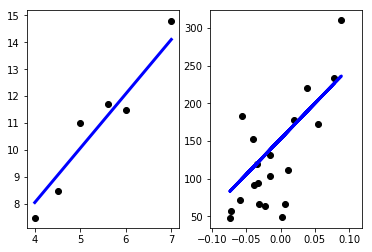
\includegraphics[height=0.3\textheight,width=0.8\linewidth]{r-squared-comparison.png}
	\caption{sample regression fits}
	\label{fig:sample regression fits}
\end{figure}

The r-squared for the regression model on the left is $93\%$ and for the model on the right it is $47\%$. When a regression model accounts for more of the variance, the data points are closer to the regression line. In practice, a regression model with $R^2$ of $100\%$ is never observed. In that case fitted values equal the data values and consequently all observation fall exactly on the regression line.

The below function can be used as a reference to implement r-squared in Rust. We first take the model variance which is the sum of the squares of consecutive difference between actual and predicted values. Then we take the mean of the actual distribution and use that to calculate the variance of the test distribution. Then we run it through the r-squared formula.

\begin{lstlisting}[caption={ml\\-utils\\/src\\/sup\_metrics\\.rs}]
fn r_squared_score(y_test: &Vec<f64>, y_preds: &Vec<f64>) -> f64 {
  let mv: f64 = y_test.iter().zip(y_preds.iter()).fold(
    0., |v, (y_i, y_i_hat)| {
      v + (y_i - y_i_hat).powi(2)
    }
  );

  let mean = y_test.iter().sum::<f64>() as f64
    / y_test.len() as f64;

  let var =  y_test.iter().fold(
    0., |v, &x| {v + (x - mean).powi(2)}
  );
  let r2: f64 = 1.0 - (mv / var);
  r2
}
\end{lstlisting}

This function should not be usable by passing the \lstinline{y_test} and \lstinline{y_pred} to get the score. Since in the examples in this chapter the \lstinline{y_test} and predicted values are in \lstinline{rusty-machine} Matrices we will probably need to do something like below.

\begin{lstlisting}[caption={chapter2\\/rustlymachine\_regression/src\\/glms\\.rs}]
println!("glm poisson R2 score: {:?}", r_squared_score(
    &boston_y_test.data(), &predictions.data()));
\end{lstlisting}
\label{sub:r_squared_error}



\label{sub:evaluation_of_rusty_machine_models}


\section{Conclusion}
This chapter introduced you to different regression algorithms such as Linear Regression, Gaussian Processes and Generalized Linear Models. Along with the algorithms, the package \lstinline{rusty_machine}  is introduced and how to create regression models of these algorithms using the package. Finally we end the chapter with an understanding of how to evaluate regression models.

In the next chapter you will learn about creating classification models.

\printbibliography
\end{document}
